% Created 2017-11-02 to 14:17
% Intended LaTeX compiler: pdflatex
\documentclass{article}

%%%% settings when exporting code %%%% 

\usepackage{listings}
\lstset{
keywordstyle=\color{blue},
commentstyle=\color{red},stringstyle=\color[rgb]{0,.5,0},
literate={~}{$\sim$}{1},
basicstyle=\ttfamily\small,
columns=fullflexible,
breaklines=true,
breakatwhitespace=false,
numbers=left,
numberstyle=\ttfamily\tiny\color{gray},
stepnumber=1,
numbersep=10pt,
backgroundcolor=\color{white},
tabsize=4,
keepspaces=true,
showspaces=false,
showstringspaces=false,
xleftmargin=.23in,
frame=single,
basewidth={0.5em,0.4em},
}

%%%% packages %%%%%

\usepackage[utf8]{inputenc}
\usepackage[T1]{fontenc}
\usepackage{lmodern}
\usepackage{textcomp}
\usepackage{color}
\usepackage{enumerate}
\usepackage{graphicx}
\usepackage{grffile}
\usepackage{wrapfig}
\usepackage{capt-of}
\usepackage{rotating}
\usepackage{caption}
\usepackage{rotating}
\usepackage{longtable}
\usepackage{multirow}
\usepackage{multicol}
\usepackage{pdflscape}
\usepackage{setspace}
\usepackage{geometry}
\usepackage{amssymb}
\usepackage{amsmath}
\usepackage{amsfonts}
\usepackage{dsfont}
\usepackage{textcomp}
\usepackage{array}
\usepackage{ifthen}
\usepackage{listings}
\usepackage{hyperref}
\usepackage{natbib}
%
%%%% additional latex commands %%%%
%
%
%%%% additional packages %%%%
%
\usepackage{authblk}
\RequirePackage{amsmath}
\RequirePackage{algorithm}
\RequirePackage[noend]{algpseudocode}
\RequirePackage{colortbl} % arrayrulecolor to mix colors
%% \input{0_Display.tex}
\RequirePackage{epstopdf} % to be able to convert .eps to .pdf image files
\RequirePackage{ifthen}
\RequirePackage{xspace} % space for newcommand macro
\RequirePackage{xifthen}
\RequirePackage{xargs}
\RequirePackage{dsfont}
\RequirePackage{amsmath,stmaryrd,graphicx}
\RequirePackage{prodint} % product integral symbol (\PRODI)
\newcommand\defOperator[7]{%
\ifthenelse{\isempty{#2}}{
\ifthenelse{\isempty{#1}}{#7{#3}#4}{#7{#3}#4 \left#5 #1 \right#6}
}{
\ifthenelse{\isempty{#1}}{#7{#3}#4_{#2}}{#7{#3}#4_{#1}\left#5 #2 \right#6}
}
}
\newcommand\defUOperator[5]{%
\ifthenelse{\isempty{#1}}{
#5\left#3 #2 \right#4
}{
\ifthenelse{\isempty{#2}}{\underset{#1}{\operatornamewithlimits{#5}}}{
\underset{#1}{\operatornamewithlimits{#5}}\left#3 #2 \right#4}
}
}
\newcommand{\defBoldVar}[2]{
\ifthenelse{\equal{#2}{T}}{\boldsymbol{#1}}{\mathbf{#1}}
}
\newcommandx\Cov[2][1=,2=]{\defOperator{#1}{#2}{C}{ov}{[}{]}{\mathbb}}
\newcommandx\Esp[2][1=,2=]{\defOperator{#1}{#2}{E}{}{[}{]}{\mathbb}}
\newcommandx\Prob[2][1=,2=]{\defOperator{#1}{#2}{P}{}{[}{]}{\mathbb}}
\newcommandx\Qrob[2][1=,2=]{\defOperator{#1}{#2}{Q}{}{[}{]}{\mathbb}}
\newcommandx\Var[2][1=,2=]{\defOperator{#1}{#2}{V}{ar}{[}{]}{\mathbb}}
\newcommandx\Binom[2][1=,2=]{\defOperator{#1}{#2}{B}{}{(}{)}{\mathcal}}
\newcommandx\Gaus[2][1=,2=]{\defOperator{#1}{#2}{N}{}{(}{)}{\mathcal}}
\newcommandx\Wishart[2][1=,2=]{\defOperator{#1}{#2}{W}{ishart}{(}{)}{\mathcal}}
\newcommandx\Likelihood[2][1=,2=]{\defOperator{#1}{#2}{L}{}{(}{)}{\mathcal}}
\newcommandx\Information[2][1=,2=]{\defOperator{#1}{#2}{I}{}{(}{)}{\mathcal}}
\newcommandx\Score[2][1=,2=]{\defOperator{#1}{#2}{S}{}{(}{)}{\mathcal}}
\newcommandx\Vois[2][1=,2=]{\defOperator{#1}{#2}{V}{}{(}{)}{\mathcal}}
\newcommandx\IF[2][1=,2=]{\defOperator{#1}{#2}{IF}{}{(}{)}{\mathcal}}
\newcommandx\Ind[1][1=]{\defOperator{}{#1}{1}{}{(}{)}{\mathds}}
\newcommandx\Max[2][1=,2=]{\defUOperator{#1}{#2}{(}{)}{min}}
\newcommandx\Min[2][1=,2=]{\defUOperator{#1}{#2}{(}{)}{max}}
\newcommandx\argMax[2][1=,2=]{\defUOperator{#1}{#2}{(}{)}{argmax}}
\newcommandx\argMin[2][1=,2=]{\defUOperator{#1}{#2}{(}{)}{argmin}}
\newcommandx\cvD[2][1=D,2=n \rightarrow \infty]{\xrightarrow[#2]{#1}}
\newcommandx\Hypothesis[2][1=,2=]{
\ifthenelse{\isempty{#1}}{
\mathcal{H}
}{
\ifthenelse{\isempty{#2}}{
\mathcal{H}_{#1}
}{
\mathcal{H}^{(#2)}_{#1}
}
}
}
\newcommandx\dpartiel[4][1=,2=,3=,4=\partial]{
\ifthenelse{\isempty{#3}}{
\frac{#4 #1}{#4 #2}
}{
\left.\frac{#4 #1}{#4 #2}\right|_{#3}
}
}
\newcommandx\dTpartiel[3][1=,2=,3=]{\dpartiel[#1][#2][#3][d]}
\newcommandx\ddpartiel[3][1=,2=,3=]{
\ifthenelse{\isempty{#3}}{
\frac{\partial^{2} #1}{\left( \partial #2\right)^2}
}{
\frac{\partial^2 #1}{\partial #2\partial #3}
}
}
\newcommand\Real{\mathbb{R}}
\newcommand\Rational{\mathbb{Q}}
\newcommand\Natural{\mathbb{N}}
\newcommand\trans[1]{{#1}^\intercal}%\newcommand\trans[1]{{\vphantom{#1}}^\top{#1}}
\newcommand{\independent}{\mathrel{\text{\scalebox{1.5}{$\perp\mkern-10mu\perp$}}}}
\author{Brice Ozenne}
\date{\today}
\title{Latent variable model and identifiability}
\hypersetup{
 pdfauthor={Brice Ozenne},
 pdftitle={Latent variable model and identifiability},
 pdfkeywords={},
 pdfsubject={},
 pdfcreator={Emacs 25.2.1 (Org mode 9.0.4)}, 
 pdflang={English}}
\begin{document}

\maketitle

\section{A necessary condition for identifiability}
\label{sec:org3f6f343}
One way to assess identifiability of a model is to count the number of parameters vs. the
number of sufficient statistics brought by the data. If the number of parameters in the
model exceed the number of sufficient statistics brought by the data the model is no more
identifiable.

\subsection{Example in univariate linear models}
\label{sec:org3dd5345}
Assuming normality of my variable, the mean and variance are
sufficient statistics (i.e. knowing the mean and the variance, I can
simulate new data following the same law as my observed data). Then I
need at least two observations to fit a linear model:

\lstset{language=r,label= ,caption= ,captionpos=b,numbers=none}
\begin{lstlisting}
set.seed(10)
data <- data.frame(Y = rnorm(10),
		   X = rnorm(10))
summary(lm(Y ~ 1, data = data[1,, drop = FALSE]))
\end{lstlisting}

\begin{verbatim}
Call:
lm(formula = Y ~ 1, data = data[1, , drop = FALSE])

Residuals:
ALL 1 residuals are 0: no residual degrees of freedom!

Coefficients:
            Estimate Std. Error t value Pr(>|t|)
(Intercept)  0.01875         NA      NA       NA

Residual standard error: NaN on 0 degrees of freedom
\end{verbatim}

\lstset{language=r,label= ,caption= ,captionpos=b,numbers=none}
\begin{lstlisting}
summary(lm(Y ~ 1, data = data[1:2,, drop = FALSE]))
\end{lstlisting}

\begin{verbatim}
Call:
lm(formula = Y ~ 1, data = data[1:2, , drop = FALSE])

Residuals:
      1       2 
 0.1015 -0.1015 

Coefficients:
            Estimate Std. Error t value Pr(>|t|)
(Intercept) -0.08275    0.10150  -0.815    0.565

Residual standard error: 0.1435 on 1 degrees of freedom
\end{verbatim}

If I also want to adjust on X, the new sufficient statistic to estimate is the covariance between
X and Y so I need at least one more observation:

\lstset{language=r,label= ,caption= ,captionpos=b,numbers=none}
\begin{lstlisting}
summary(lm(Y ~ X, data = data[1:2,, drop = FALSE]))
\end{lstlisting}

\begin{verbatim}
Call:
lm(formula = Y ~ X, data = data[1:2, , drop = FALSE])

Residuals:
ALL 2 residuals are 0: no residual degrees of freedom!

Coefficients:
            Estimate Std. Error t value Pr(>|t|)
(Intercept)  -0.6277         NA      NA       NA
X             0.5867         NA      NA       NA

Residual standard error: NaN on 0 degrees of freedom
Multiple R-squared:      1,	Adjusted R-squared:    NaN 
F-statistic:   NaN on 1 and 0 DF,  p-value: NA
\end{verbatim}

\lstset{language=r,label= ,caption= ,captionpos=b,numbers=none}
\begin{lstlisting}
summary(lm(Y ~ X, data = data[1:3,, drop = FALSE]))
\end{lstlisting}

\begin{verbatim}
Call:
lm(formula = Y ~ X, data = data[1:3, , drop = FALSE])

Residuals:
       1        2        3 
-0.07153  0.09643 -0.02490 

Coefficients:
            Estimate Std. Error t value Pr(>|t|)  
(Intercept) -1.09101    0.09767 -11.171   0.0568 .
X            1.07216    0.12465   8.602   0.0737 .
---
Signif. codes:  0 '***' 0.001 '**' 0.01 '*' 0.05 '.' 0.1 ' ' 1

Residual standard error: 0.1226 on 1 degrees of freedom
Multiple R-squared:  0.9867,	Adjusted R-squared:  0.9733 
F-statistic: 73.99 on 1 and 1 DF,  p-value: 0.07368
\end{verbatim}

\section{Application to latent variable models (lvm)}
\label{sec:org68b96b5}

In a latent variable model things are simular. Because we are interested in modeling the
relationship between variables, usually we focus on the covariance matrix: does the observed
covariance matrix enable to identify the modeled covariance matrix? 

\subsection{Example: lvm with bivariate outcome}
\label{sec:org8e5bde5}
Consider the following model:

\lstset{language=r,label= ,caption= ,captionpos=b,numbers=none}
\begin{lstlisting}
library(lava)

lvm.2Y <- lvm(c(Y, E) ~ eta)
lvm.2Y <- latent(lvm.2Y, "eta")
\end{lstlisting}

\begin{center}
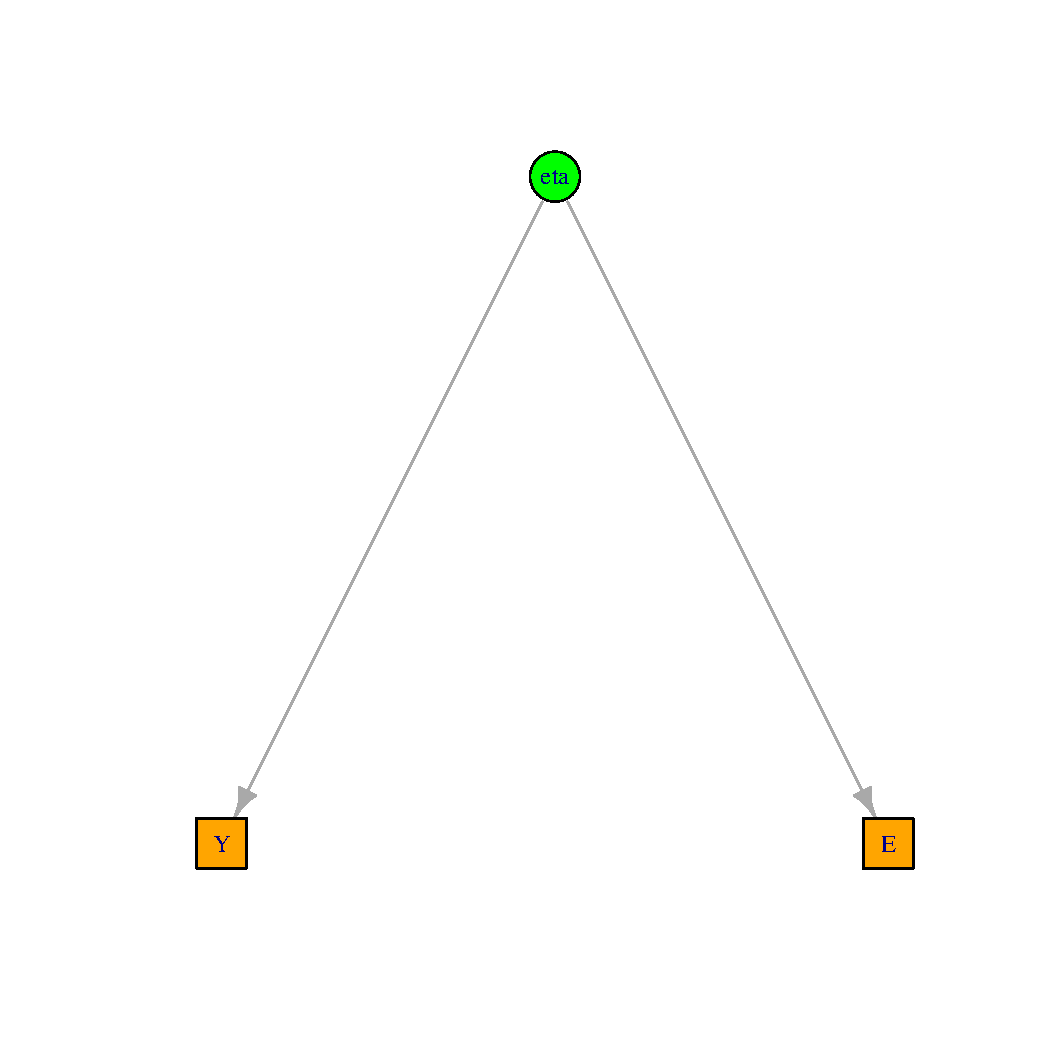
\includegraphics[width=0.5\textwidth]{./figures/show-bivariateLVM.pdf}
\end{center}

This model involves 3 variables (2 observed and 1 latent). We can
write the \textbf{full variance-covariance matrix} between all the variables:
\begin{align*}
\Sigma_{Y,\eta,E} = \begin{bmatrix} 
\Var(Y) & \Cov(Y,\eta) & \Cov(Y,E) \\ & \Var(\eta) & \Cov(\eta,E) \\ & & \Var(E)  \\
\end{bmatrix} 
\end{align*}

The \textbf{empirical variance-covariance matrix} only contains three different parameters:
\begin{align*}
S = 
\begin{bmatrix} 
\Var(Y) & \Cov(Y,E) \\ & \Var(E) \\
\end{bmatrix} 
\end{align*}
We can check that in R:
\lstset{language=r,label= ,caption= ,captionpos=b,numbers=none}
\begin{lstlisting}
n <- 1e3
df.2Y <- sim(lvm.2Y, n, latent = FALSE)
cov(df.2Y)
\end{lstlisting}

\begin{verbatim}
         Y        E
Y 2.070255 1.112335
E 1.112335 2.138186
\end{verbatim}


By default lava parametrize the \textbf{modeled variance-covariance matrix},
setting some covariance links to a fixed value. In lava notations, we
have:
\begin{align*}
\theta = \left(Y \sim\sim Y, \eta \sim\sim \eta, E \sim \eta, E \sim\sim E\right)
\end{align*}
We therefore need to estimate the 4 parameters from the empirical
covariance matrix.

For the mean parameters the full expectation vector would contain 3
parameters, one for each variable. We only observe two of them (\(Y\)
and \(E\)) and by default lava fix the intercept of \(Y\) to be 0 so
there are only two mean parameters. 

In total we have 6 parameters to estimate (2 mean, 4
variance-covariance) but can only estimate 5 empirical moments (2
mean, 3 variance-covariance). The model is therefore not identifiable.
This means that the lvm won't properly converge:
\lstset{language=r,label= ,caption= ,captionpos=b,numbers=none}
\begin{lstlisting}
estimate(lvm.2Y, data = df.2Y)
\end{lstlisting}

\begin{verbatim}
                       Estimate  Std. Error     Z-value P-value
Measurements:                                                  
   E~eta             1.2791e+00  2.3246e+06  0.0000e+00       1
Intercepts:                                                    
   E                 1.4000e-03  2.9136e+04  0.0000e+00       1
   eta              -1.2530e-02  4.5480e-02 -2.7561e-01  0.7828
Residual Variances:                                            
   Y                 1.1994e+00  1.5788e+06  0.0000e+00        
   E                 7.1466e-01  2.5832e+06  0.0000e+00        
   eta               8.6874e-01  1.5788e+06  0.0000e+00
\end{verbatim}

The non identifiability come from the fact that the only equation
defining the parameters \(E \sim eta\) and \(\eta \sim \sim \eta\) is:
\begin{align*}
\Cov[Y,E] &= (E \sim eta) * (\eta \sim \sim \eta)
\end{align*}
This is clearly not identifiable: \(E \sim eta\) and \(Y \sim eta\) need to be constrained to be 1.
\lstset{language=r,label= ,caption= ,captionpos=b,numbers=none}
\begin{lstlisting}
lvm.2Y.constrain <- lvm.2Y
regression(lvm.2Y.constrain,E~eta) <- 1
regression(lvm.2Y.constrain,Y~eta) <- 1
estimate(lvm.2Y.constrain, data = df.2Y)
\end{lstlisting}

\begin{verbatim}
                    Estimate Std. Error  Z-value P-value
Intercepts:                                             
   E                -0.00210    0.04452 -0.04718  0.9624
   eta              -0.01253    0.04548 -0.27561  0.7828
Residual Variances:                                     
   Y                 0.95696    0.07081 13.51394        
   E                 1.02482    0.07269 14.09907        
   eta               1.11122    0.07518 14.78015
\end{verbatim}

\subsection{Example 2: lvm with bivariate outcome with group effect}
\label{sec:orgc4cc5b6}
Let's modify the previous model by adding an exogenous variable
affecting the latent variable:

\lstset{language=r,label= ,caption= ,captionpos=b,numbers=none}
\begin{lstlisting}
lvm.2Y.Age <- lvm.2Y
regression(lvm.2Y.Age) <- eta~Age
\end{lstlisting}

\begin{center}
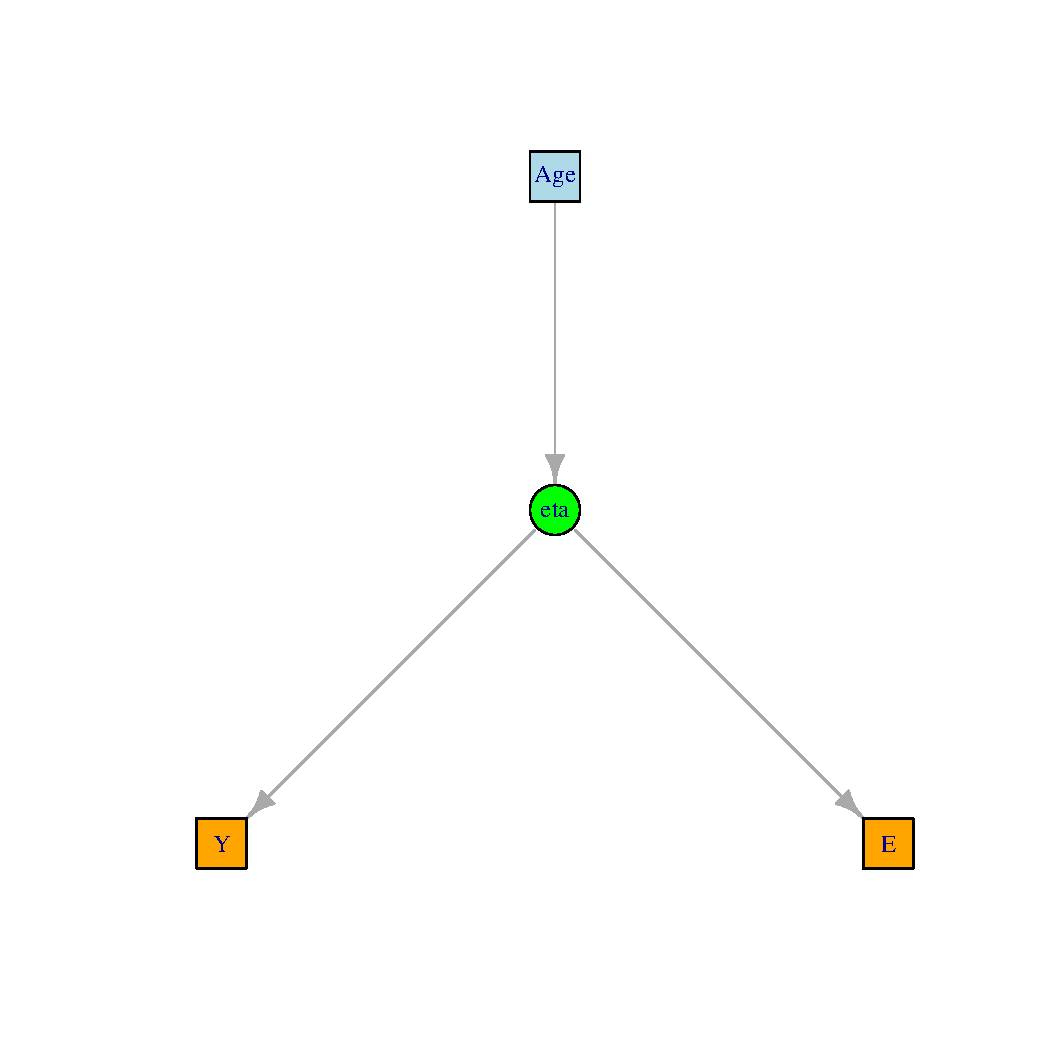
\includegraphics[width=0.5\textwidth]{./figures/show-bivariateLVM-Age.pdf}
\end{center}

The new \textbf{modeled variance-covariance matrix} contains 6 parameters:
\begin{align*}
\theta = \left( Y \sim \sim Y,  \eta \sim \sim \eta, E \sim \eta, \eta \sim Age, E \sim \sim E, Age \sim \sim Age \right)
\end{align*}
while the new \textbf{empirical variance-covariance matrix} contains 6 parameters:
\begin{align*}
S = 
\begin{bmatrix} 
\Var(Y) & \Cov(Y,E) & \Cov(Y,Age) \\ & \Var(E) & \Cov(E,Age) \\ && \Var(Age) \\
\end{bmatrix} 
\end{align*}
So the model satisfy one necessary condition for being
identifiable. This condition is however not sufficient to ensure
identifiability but is easier to check than the NSC (nessary and
sufficient condition). To check the NSC we need to write down the
equations relating the empirical and the theoretical moments:
\begin{align*}
\Var(Y) &= Y \sim \sim Y + \eta \sim \sim \eta \\
\Var(E) &= E \sim \sim E + (E \sim \eta) * (\eta \sim \sim \eta) \\
\Var(Age) &= Age \sim \sim Age \\
\Cov(Y,E) &= (E \sim \eta) * (\eta \sim \sim \eta) \\
\Cov(Y,Age) &= (\eta \sim Age) * (Age \sim \sim Age) \\
\Cov(E,Age) &= (E \sim \eta) * (\eta \sim Age) * (Age \sim \sim Age) \\
\end{align*}
We can re-writte that in matricial form:
\begin{align*}
\begin{bmatrix}
\Var(Y) \\
\Var(E) \\
\Var(Age) \\
\Cov(Y,E) \\
\Cov(Y,Age) \\
\Cov(E,Age) \\
\end{bmatrix}
& = \begin{bmatrix}
1&0&1&0&0&0\\
0&1&1&0&1&0\\
0&0&0&1&0&0\\
0&0&1&0&1&0\\
0&0&0&1&0&1\\
0&0&0&1&1&1\\
\end{bmatrix}
\begin{bmatrix}
Y \sim \sim Y \\
E \sim \sim E \\
\eta \sim \sim \eta \\
Age \sim \sim Age \\
E \sim \eta \\
\eta \sim Age \\
\end{bmatrix} \\
b &= X \theta
\end{align*}
This problem is identifiable if and only if \(X\) has non-zero eigenvalues:
\lstset{language=r,label= ,caption= ,captionpos=b,numbers=none}
\begin{lstlisting}
X <- rbind(c(1,0,1,0,0,0),
c(0,1,1,0,1,0),
c(0,0,0,1,0,0),
c(0,0,1,0,1,0),
c(0,0,0,1,0,1),
c(0,0,0,1,1,1))
svd(X)$d
\end{lstlisting}

\begin{verbatim}
[1] 2.4825297 2.0685860 1.2223636 0.7442566 0.6272682 0.3412366
\end{verbatim}

Therefore the model is identifiable.

This is confirmed by the fact that lava is able to estimate the model:
\lstset{language=r,label= ,caption= ,captionpos=b,numbers=none}
\begin{lstlisting}
df.2Y.Age <- sim(lvm.2Y.Age, n = n)
estimate(lvm.2Y.Age, data = df.2Y.Age)
\end{lstlisting}

\begin{verbatim}
                    Estimate Std. Error  Z-value  P-value
Measurements:                                            
   E~eta             0.98049    0.04851 20.21039   <1e-12
Regressions:                                             
   eta~Age           0.99614    0.04703 21.18155   <1e-12
Intercepts:                                              
   E                 0.00459    0.04627  0.09910   0.9211
   eta               0.01963    0.04505  0.43568   0.6631
Residual Variances:                                      
   Y                 1.00969    0.08979 11.24480         
   E                 1.16935    0.09111 12.83393         
   eta               1.01691    0.08995 11.30476
\end{verbatim}

Compared to the previous example two equations now define the parameters \(E \sim
eta\) and \(\eta \sim \sim \eta\):
\begin{align*}
\Cov[Y,E] &= (E \sim eta) * (\eta \sim \sim \eta) \\
\Cov[E,Age] &= (E \sim eta) * (\eta \sim Age) * (Age \sim \sim Age)
\end{align*}

Note that the model is exactly identifiable in the sense that we have
exactly the same number of parameters and moments. Adding an
additional link between age and one outcome would make the model non
identifiable since we would increase by one the number of parameters
(p=7) while still having only 6 moments.

\lstset{language=r,label= ,caption= ,captionpos=b,numbers=none}
\begin{lstlisting}
lvm.2Y.Age2 <- lvm.2Y.Age
regression(lvm.2Y.Age2) <- Y~Age
\end{lstlisting}

\begin{center}
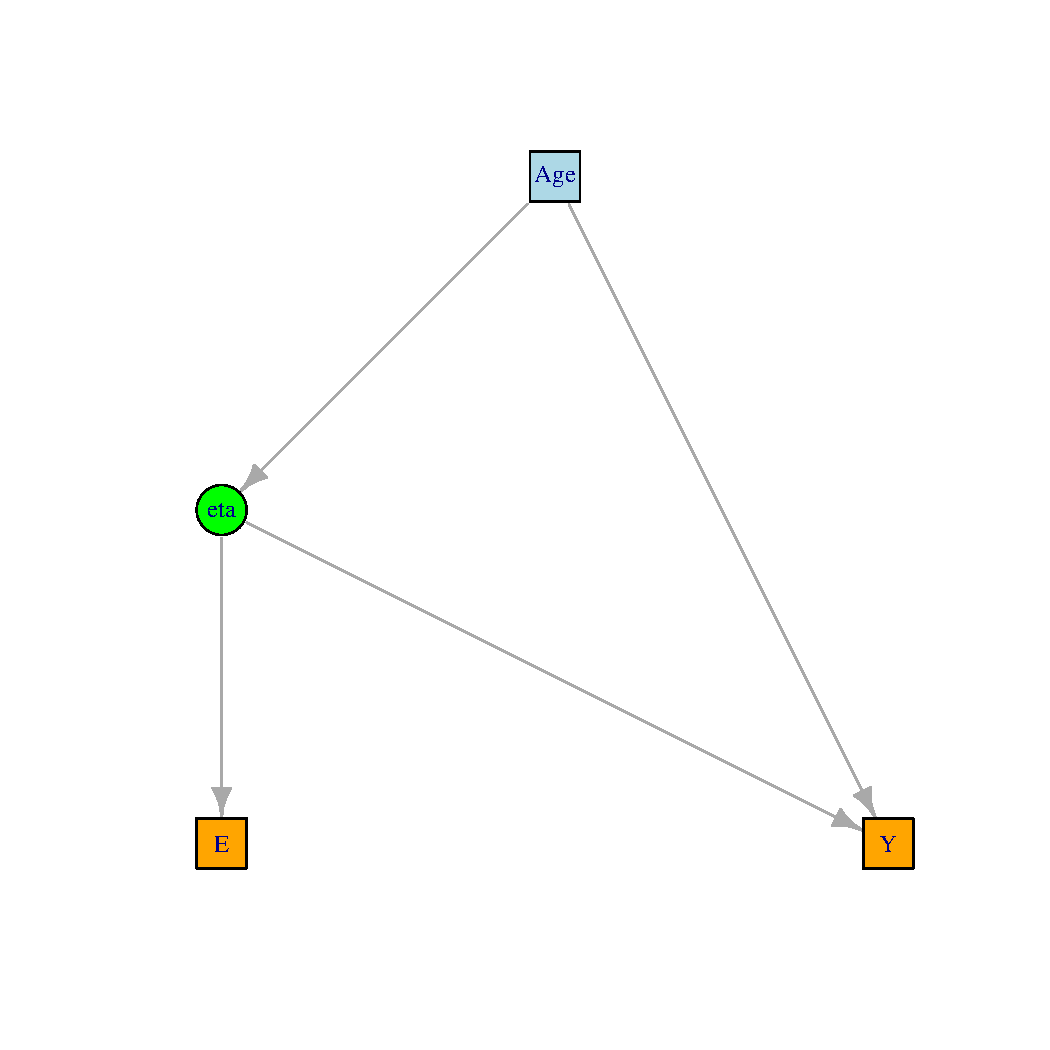
\includegraphics[width=0.5\textwidth]{./figures/show-bivariateLVM-Age2.pdf}
\end{center}

Indeed lava is not able to estimate the model:
\lstset{language=r,label= ,caption= ,captionpos=b,numbers=none}
\begin{lstlisting}
df.2Y.Age2 <- sim(lvm.2Y.Age2, n = n)
estimate(lvm.2Y.Age2, data = df.2Y.Age2)
\end{lstlisting}

\begin{verbatim}
                       Estimate  Std. Error     Z-value P-value
Measurements:                                                  
   E~eta             1.4091e+00  2.1518e+06  0.0000e+00       1
Regressions:                                                   
   Y~Age             1.2775e+00  1.1396e+06  0.0000e+00       1
    eta~Age          7.4624e-01  1.1396e+06  0.0000e+00       1
Intercepts:                                                    
   E                -5.1720e-02  1.1079e+05  0.0000e+00       1
   eta               5.1490e-02  4.4290e-02  1.1624e+00  0.2451
Residual Variances:                                            
   Y                 1.2724e+00  1.0436e+06  0.0000e+00        
   E                 6.4440e-01  2.0722e+06  0.0000e+00        
   eta               6.8340e-01  1.0436e+06  0.0000e+00
\end{verbatim}
\end{document}